\documentclass[10pt,a4paper]{article}
\usepackage[a4paper, left=3cm, right=3cm, top=3cm, bottom=3cm, headsep=10mm, footskip=12mm]{geometry}
\usepackage[T1]{fontenc}
\usepackage[ngerman, english]{babel}    % mehrsprachiger Textsatz
% babel: letzte Sprache in Optionen zeigt die Sprache des Dokumentes
% und kann durch den Befehl \selectlanguage{} geaendert werden
% Passen Sie die Optionen des babel-Paketes nach Bedarf an!
\usepackage{float}
\usepackage{graphicx}
\usepackage{url}
\usepackage{pdflscape}
\usepackage{mathtools}
\usepackage{amssymb, amsmath, amstext}
\usepackage{amsthm}
\usepackage{xcolor}
\usepackage{nameref}
\usepackage{siunitx}
\usepackage{makecell}
\usepackage{hyperref}
\usepackage{enumitem}
\usepackage[superscript,biblabel]{cite}
\usepackage{caption}
\usepackage{subcaption}
\usepackage{tabularx} 			% Tabellen erzeugen
\usepackage{multirow}			 % Zeilen in Tabellenbearbeitung
\usepackage{multicol} 			% Spalten in Tabellenbearbeitung 
\usepackage{lmodern}                        % Ersatz fuer Computer Modern-Schriften 
\usepackage{amsmath}                                           % zum besseren Aussehen am Bildschirm
\usepackage{booktabs} % für schönere Tabellen
\usepackage{sidecap}
\usepackage{rotating} % für die Landscape-Umgebung
\usepackage{afterpage}
\definecolor{Bluetitle}{HTML}{1F3864}
\definecolor{softbluetitle}{HTML}{274D7E}
\definecolor{Greyish}{HTML}{5A5A5A}
\renewcommand{\refname}{Reference}
\usepackage{array,multirow}
\newcommand{\specialcell}[2][c]{%
	\begin{tabular}[#1]{@{}c@{}}#2\end{tabular}}




\begin{document}
	
	\begin{titlepage}
		\begin{center}
			\begin{figure}[h!tbp]
				
\includegraphics[width=\linewidth]{HUlogo.PNG}
			\end{figure}
			\vspace*{2 cm}
			
			\textcolor{Bluetitle}{\textbf{\huge Hormone und Blütenentwicklung am Arabidopsis thalinana}}\par
			\vspace*{0.5cm}
			\textcolor{softbluetitle}{\textbf{\Large Untersuchung von Auxin- und Cytokininaktivität in der Pflanzenentwicklung und der Einfluss von ABC-Genen in der Blütenentwicklung im Modell Arabidopsis thalinana}}\par
			
			\vspace*{2cm}
			
			\textcolor{Greyish}{\textbf{Versuchsdurchführende}}\par
			\textcolor{Greyish}{Oscar Moore (634083)}\par
			\textcolor{Greyish}{Fridolin Rehning (625757)}\par
			\textcolor{Greyish}{Philipp Kunze (625468)}\par
			\textcolor{Greyish}{Daniel Kollenkirchen (625426)}\par
			\textcolor{Greyish}{Huyen Anh Nguyen (572309)}\par
			
			\vspace*{0.5cm}
			\textcolor{Greyish}{\textbf{Versuchsort}}\par
			\textcolor{Greyish}{Campus Nord, Haus 9}\par
			\textcolor{Greyish}{R2006}\par
			\vspace*{0.5cm}
			\textcolor{Greyish}{\textbf{Versuchsbetreuer}}\par
			\textcolor{Greyish}{Dr. Cezary Smaczniak}\par
			
			\vspace*{2 cm}
			
			\textcolor{Greyish}{18. Juni 2024}\par
			
			
			
			
		\end{center}
	\end{titlepage}
	
	\tableofcontents
	
	\section{Einführung}	
	
	\section{Material und Methode}
	Wildtyp und 5 verschiedene Mutanten der Pflanze Arabidopsis thalinana wurde in diesen Versuch verwendet.
	\subsection{Histochemische Färbung der Auxin- und Cytokininaktivität}
	In  diesem Versuch sollte die Cytokinin und Auxin Antwort, in verschiedenen Geweben,  histochemisch ermittelt werden. Verwendet wurden transgene Pflanzen , in denen Auxin / Cytokinin abhängige Sequenzen mit ß-Glucuronidase-Reportergenen (GUS) gekoppelt waren. Bei der regulatorischen Sequenz, welche die Aktivität der Auxinantwort misst, handelt es sich um den sogenannten DR5-Promotor. Bei der regulatorischen Sequenz, welche die Aktivität der Cytokininantwort misst, handelt es sich um den sogenannten TCS-Promotor.\\
	Um die GUS-Färbelösung herzustellen, mussten zuerst die Konzentrationen der Komponenten berechnet werden. Hierbei  wurden folgende  Werte ermmittelt:
	\begin{itemize}
		\item 100 $\mu$L Ferrocyanid-Stammlösung
		\item 100 $\mu$L Ferricyanid-Stammlösung
		\item 800 $\mu$L Phosphatpuffer
	\end{itemize}
	Anschließend  wurde  die Färbelösung in ein 1,5ml Reaktionsgefäß pipettiert, indem bereits 1mg  X-Gluc vorabgewogen enthalten war. Mithilfe einer Glaspasteurpipette  wurde dann noch ein Tropfen Triton-X-100 hinzugegeben und dann solange gevortext, bis das X-Gluc sich vollkommen  aufgelöst hat.\\
	Für die Färbung wurden 1-2 Blätter, sowie Schoten in ein 1,5ml Reaktionsgefäß getan und vorsichtig mit 300$\mu$L GUS-Färbelösung hinzupipettiert. Das Reaktionsgefäß wurde offen auf Eis in die  Eppendorf Vakuumfuge gestellt und 5min infiltriert. Da das Reaktionsgefäß anschließend über Nacht bei 37°C inkubiert, haben wir  im nächsten Schritt mit dem Proben  von der Gruppe vom Vortag weitergearbeitet.\\
	Bei der Entfärbung wurde die GUS-Färbelösung zunächst abpipettiert. Unterm Abzug wurden dann 500$\mu$L Ethanol-Essigsäure-Mix in das Reaktionsgefäß gegeben. Da auch hier das Entfärben über Nacht passierte, wurde anschließend eine Probe  einer  anderen  Gruppe Stereomikroskopisch analysiert. Hierzu wurde die entfärbte Probe auf einem Objektträger Platziert und tropfenweise Ethanol (70$\%$) hinzugegeben. Es wurde festgehalten, wo die Färbung aufgetreten ist.
	\subsection{morphologische Beurteilung der Mutation anhand der Blütenbildung}
	Es wurde phänotypisch die Blütenblätter der Mutanten 1 bis 5 unter einem Stereomikroskop untersucht.
	
	\section{Ergebnis}
	
	\subsection{Auxin- und Cytokininaktivität}
		\subsubsection{Auxinaktivität}

		\subsubsection{Cytokininaktivität}
		Mittels GUS-Färbung konnten die Gewebeteile, die eine Cytokinin (CK)-Aktivität zeigen, angefärbt werden. Nach Betrachtung unter dem Stereo-Mikroskop ist zu erkennen, dass vor allem die Leitbündel der Blätter eine Färbung zeigten (Figure \ref{fig:cytokinin_TCS_Färbung}, Rechts). Die Infloreszenzen hingegen zeigten eine starke Färbung in den Blütenböden, die als kleine Punkte sichtbar waren. (siehe Figure \ref{fig:cytokinin_TCS_Färbung}, links). Bei der Frucht (Schote) konnte keine eindeutige Färbung ausgemacht werden. Es konnte jedoch eine leichte Zunahme der Färbung von der Narbe hin zum Fruchtstiel, beobachtet werden (siehe Figure \ref{fig:cytokinin_TCS_Färbung} Mitte).\\
		Anhand der zur Verfügung gestellten Dauerpräparate konnte man ebenfalls die CK-Aktivität in anderen Pflanzenteilen erkennen. Hier waren vor allem die Wurzeln stark gefärbt (siehe Figure \ref{fig:cytokinin_Dauerpräparat}). Zusätzlich zeigte sich, wie auch in der vorherigen Probe eine Färbung der Leitbündel der Blätter. 
		\begin{figure}[H]
			\centering
			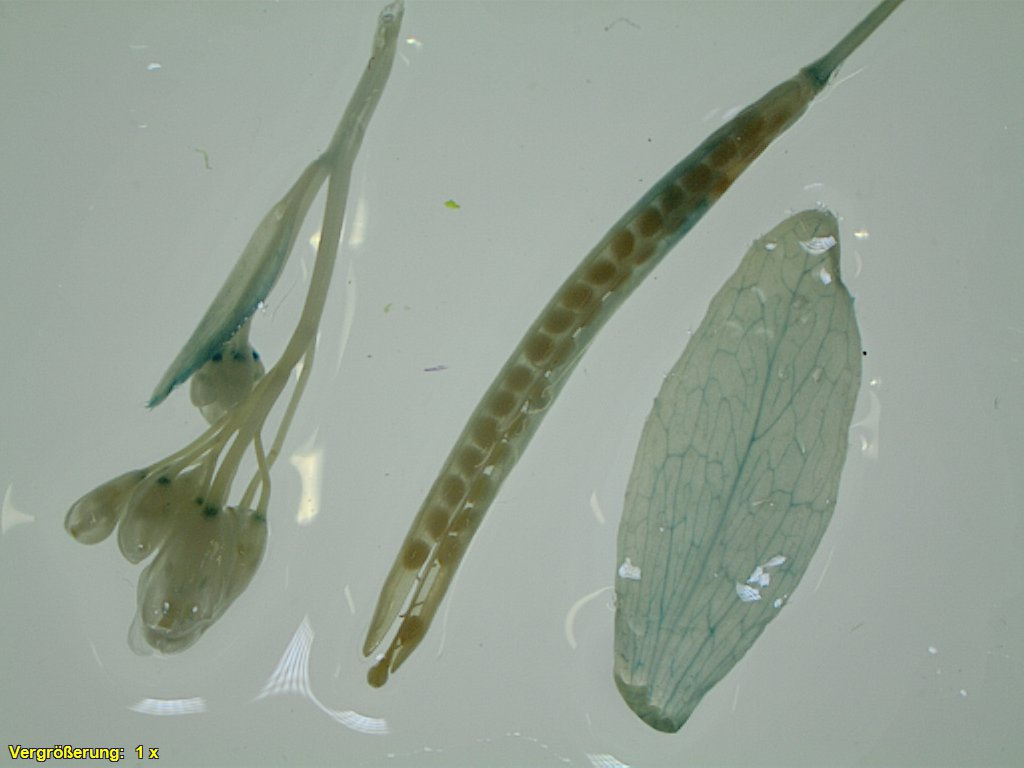
\includegraphics[scale=0.3]{TCS_O+A.jpg}
			\caption{Mit GUS-Färbung angefärbte Infloreszenzen, Schote und Blatt von transgener Arabidopsis thaliana (mit TCS-Reportergen)}
			\label{fig:cytokinin_TCS_Färbung}
		\end{figure}	
		
			\begin{figure}[H]
			\centering
			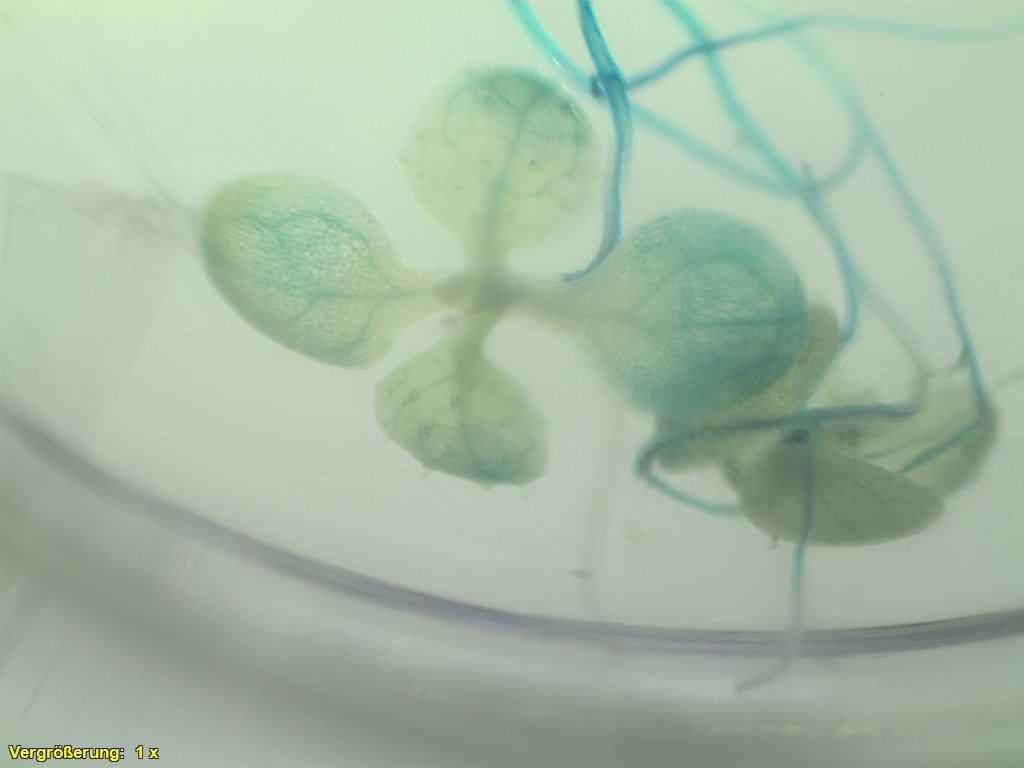
\includegraphics[scale=0.3]{TCS_DP_O+A.jpg}
			\caption{Fertigpräparate von transgenen A. thaliana Keimlingen (TCS-Reportergen), gefärbt mit GAU-Färbung}
			\label{fig:cytokinin_Dauerpräparat}
		\end{figure}	
	\subsection{Phänotypische Analyse der Blüte}
	
		\begin{figure}[H]
			\centering
			\begin{subfigure}[b]{0.45\textwidth}
				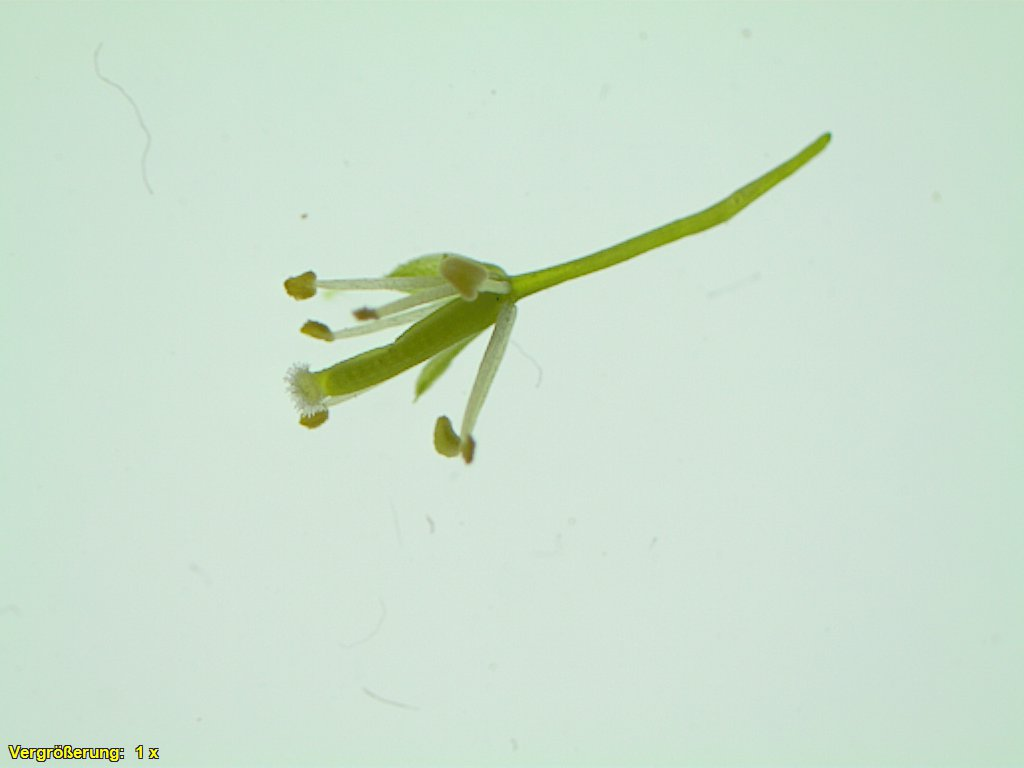
\includegraphics[width=\textwidth]{1_O+A.jpg}
				\caption{Mutant 1}
				\label{fig:M1}
			\end{subfigure}
			\hfill
			\begin{subfigure}[b]{0.45\textwidth}
				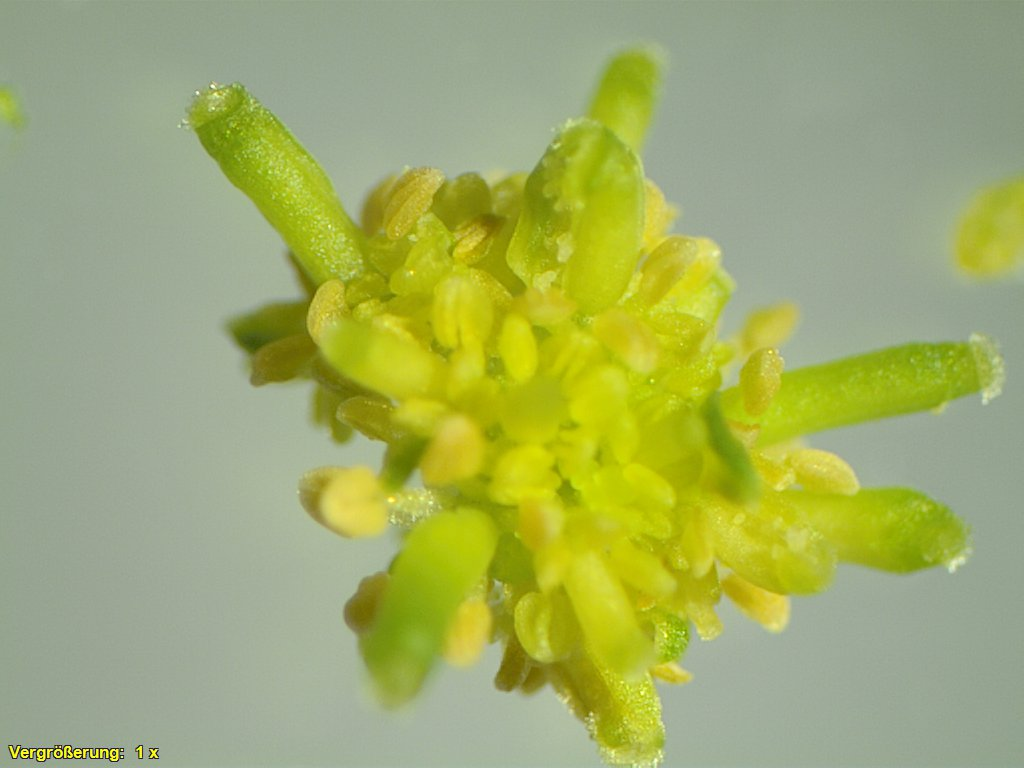
\includegraphics[width=\textwidth]{2_O+A(1).jpg}
				\caption{Mutant 2}
				\label{fig:M2}
			\end{subfigure}
			\hfill
			\begin{subfigure}[b]{0.45\textwidth}
				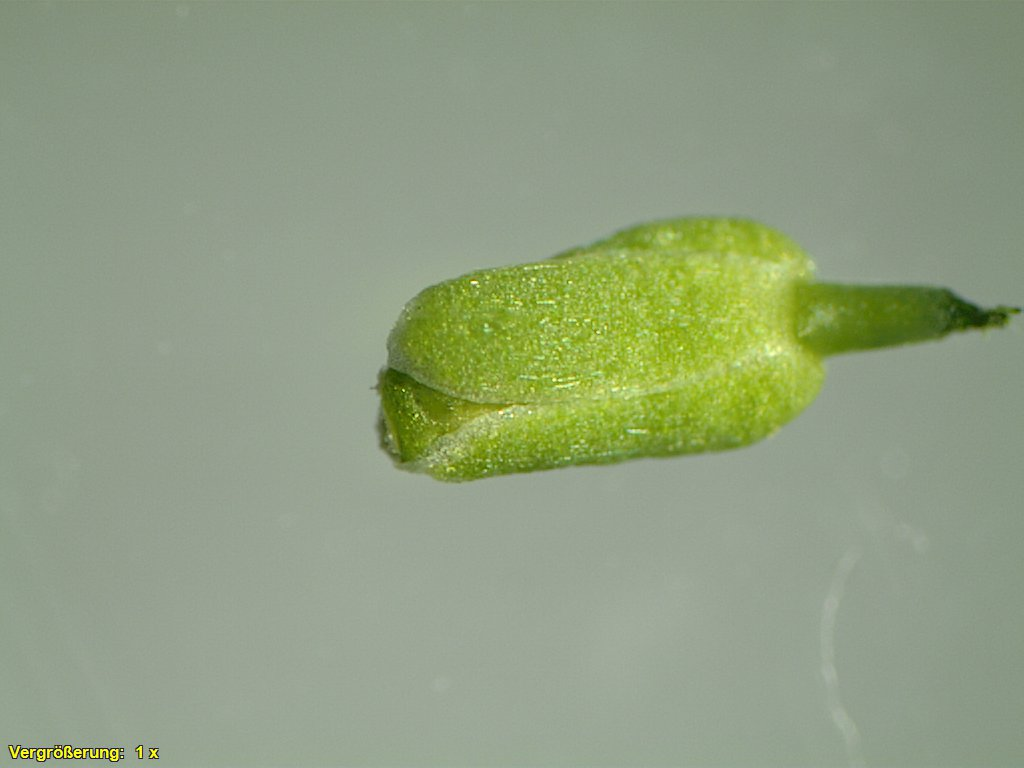
\includegraphics[width=\textwidth]{3_O+A(MU).jpg}
				\caption{Mutant 3}
				\label{fig:M3}
			\end{subfigure}
			\hfill
			\begin{subfigure}[b]{0.45\textwidth}
				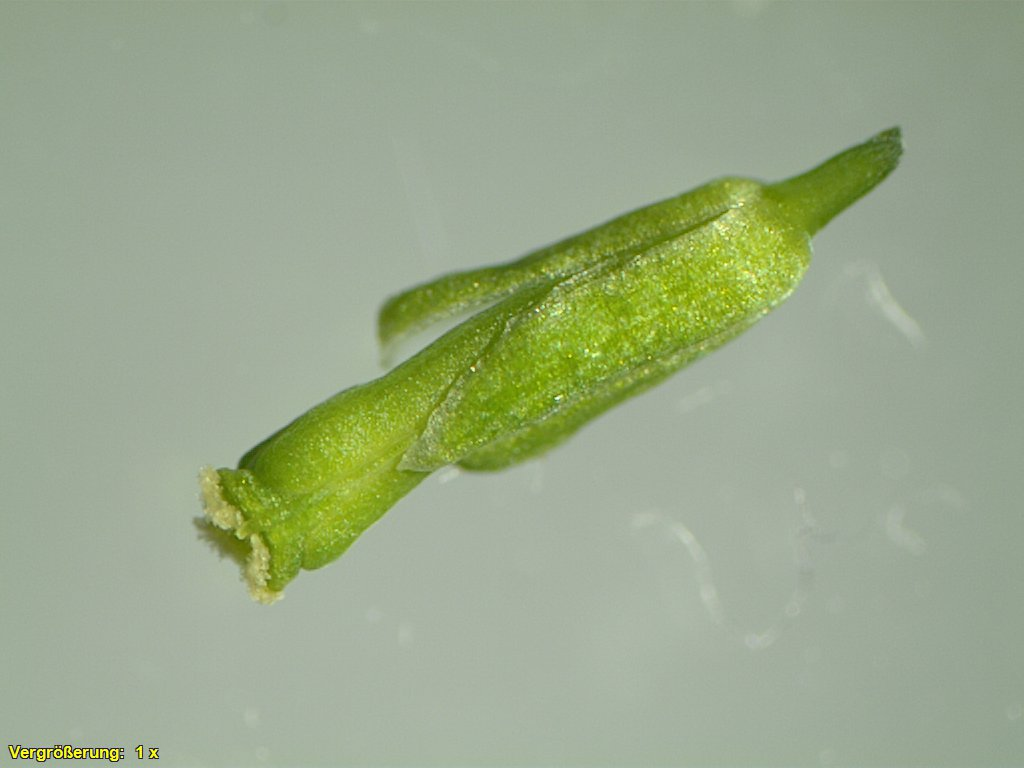
\includegraphics[width=\textwidth]{4_O+A(MU).jpg}
				\caption{Mutant 4}
				\label{fig:M4}
			\end{subfigure}
			\hfill
			\begin{subfigure}[b]{0.45\textwidth}
				\centering
				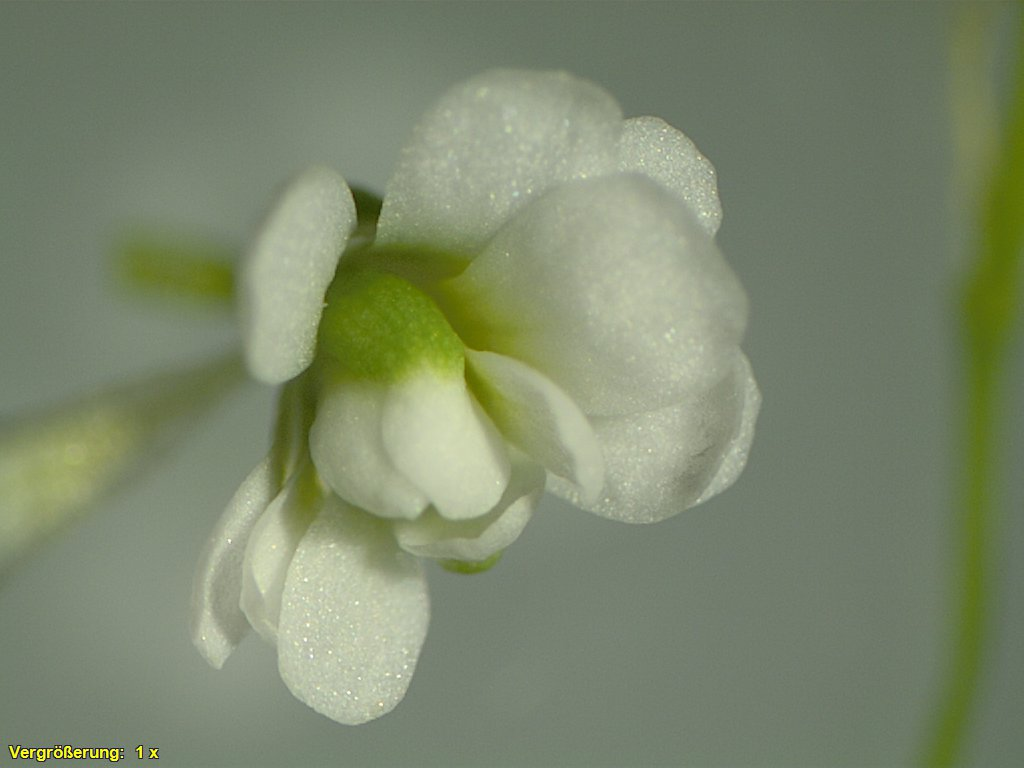
\includegraphics[width=\textwidth]{5_O+A(MU).jpg}
				\caption{Mutant 5}
				\label{fig:M5}
			\end{subfigure}
			\caption{Stereomikroskopische Aufnahme der Blüten von der Arabidopsis thalinana Mutanten 1-5 in der 1x-Vergrößerung}
		\end{figure}
		
		Die erste Mutante besitzt Staubblätter und Fruchtblätter (siehe Figure \ref{fig:M1}).
		Die zweite Mutante besitzt ebenfalls nur Staubblätter und Fruchtblätter (siehe Figure \ref{fig:M2}).\\
		In Figure \ref{fig:M3} ist in der dritten Mutante zu sehen, dass die Fruchtblätter nur von Kelchblätter umgeben ist, welches phänotypisch auch Mutant 4 vorweist (siehe Figure \ref{M4}).\\
		Die fünfte Mutante besitzt Kelchblätter, die in Figure \ref{fig:M5} nicht gut zu sehen ist und Kronenblätter.
		

	\section{Diskussion}
	
	\subsection{Floral homöotische Gene}
	
		\begin{figure}[H]
			\centering
			
\includegraphics[scale=0.85]{Wildtyp_diagramm.png}
			\caption{ABC-Modell desFloral homöotische Gen als Diagramm des Wildtypes und Blütendiagramm vom Arabidopsis thalinana.\\
			Kr = Krone, Ke = Kelch, St = Staub, Fr = Frucht -Blätter}
			\label{fig:floralgene_Wildtyp}
		\end{figure}
	
		\begin{figure}[H]
			\centering
			\begin{subfigure}[b]{0.25\textwidth}
				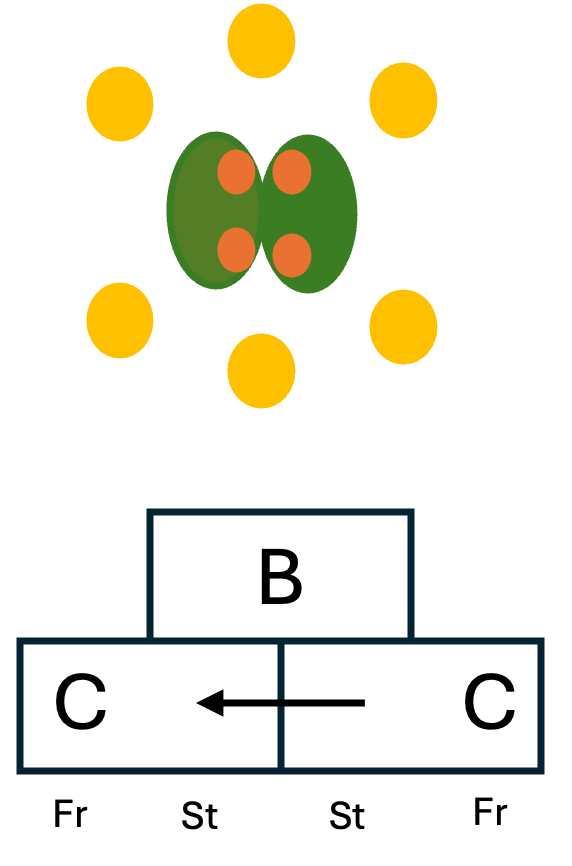
\includegraphics[width=\textwidth]{A-Typ_diagramm.png}
				\caption{A$\ominus$-Mutant}
				\label{fig:A-Mutant}
			\end{subfigure}
			\hfill
			\begin{subfigure}[b]{0.3\textwidth}
				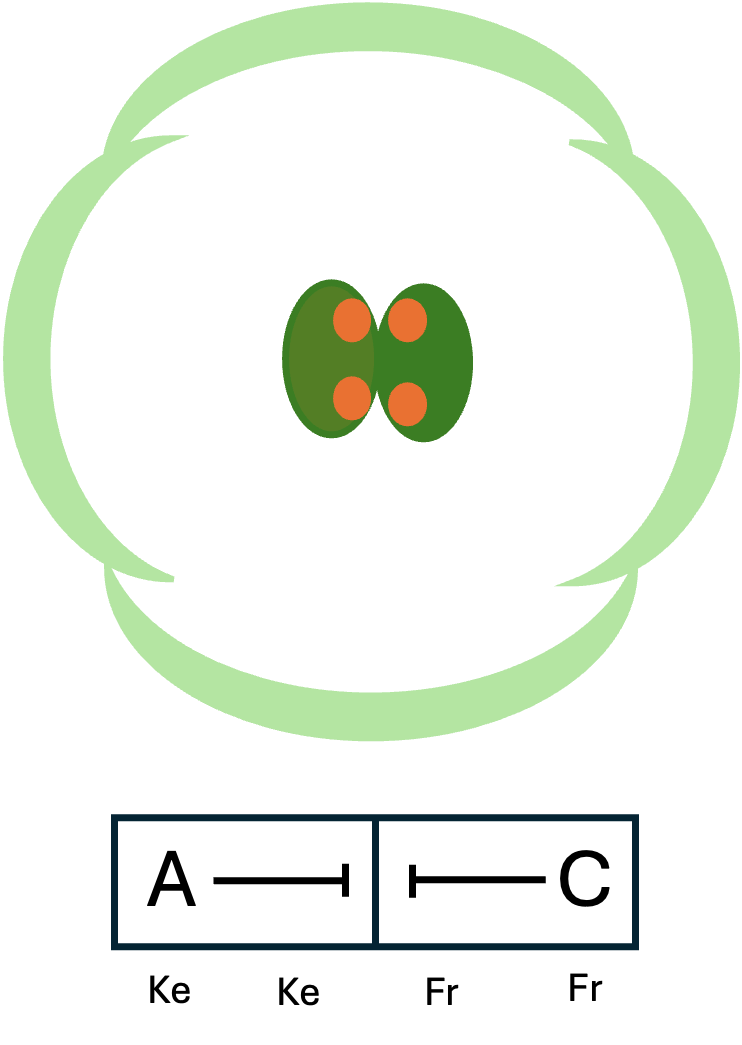
\includegraphics[width=\textwidth]{B-Mutant_diagramm.png}
				\caption{B$\ominus$-Mutant}
				\label{fig:B-Mutant}
			\end{subfigure}
			\hfill
			\begin{subfigure}[b]{0.3\textwidth}
				\includegraphics[width=\textwidth]{C-Mutant_diagramm.png}
				\caption{C$\ominus$-Mutant}
				\label{fig:C-Mutant}
			\end{subfigure}
	
			\caption{Stereoikroskopische Aufnahme der Blüten von der Arabidopsis thalinana Mutanten 1-5 in der 1x-Vergrößerung}
		\end{figure}
		
		

	\section{Anhang}

	

	
\end{document}